%%%%%%%%%%%%%%%%%%%%%%%%%%%%%%%%%%%%%%%%%%%%%%%%%%%%%%%%%%%%%%%%%%%%%%%%%%%

\documentclass{standalone}

\usepackage{mathptmx}
\usepackage{tikz}
\usetikzlibrary{angles}
\usetikzlibrary{external}
\usetikzlibrary{quotes}
\tikzexternalize{quadrant-generic-point}

%% We default to Times.
\renewcommand{\rmdefault}{ptm}
\renewcommand{\ttdefault}{pcr}
%% Enable Times/Palatino main text font.
\normalfont\selectfont

\newcommand{\comma}{,\,}
\newcommand{\tuple}[2]{\left( {#1}\comma {#2} \right)}

%% The horizontal and vertical axes.
\newcommand{\cartesianAxes}{%%
  %% The horizontal axis.
  \draw[axisStyle] (\xlow,0) -- (\xhigh,0);
  \node at (\xhigh,0) [right] {$x$};
  %% The vertical axis.
  \draw[axisStyle] (0,\ylow) -- (0,\yhigh);
  \node at (0,\yhigh) [above] {$y$};
}

%% A quadrant of the unit circle.
\newcommand{\myQuadrant}{%%
  %% Draw the quadrant.
  \draw[lineStyle] (A) arc (\angleStart:\angleEnd:\radius) -- (origin) -- cycle;
  %% Label some special points.
  \xyPoint{origin}{\tuple{0}{0}}{below right}
  \xyPoint{A}{A = \tuple{1}{0}}{below left}
  \xyPoint{%%
    B%%
  }{%%
    B = \tuple{%%
      \cos \frac{\pi}{2k}%%
    }{%%
      \sin \frac{\pi}{2k}%%
    }%%
  }{%%
    right%%
  }
  \xyPoint{C}{\tuple{0}{1}}{below right}
  %% A generic angle.
  \draw[dashStyle] (origin) -- (B);
  \path pic["$\frac{\pi}{2k}$",draw,->,thick,angle radius=1.3cm] {angle=A--origin--B};
}

%% Label a point.
%%
%% #1 -- The x- and y-coordinates.
%% #2 -- Label the point with this name.
%% #3 -- Where to place the point.
\newcommand{\xyPoint}[3]{%%
  \node[nodeStyle] at (#1) {};
  \node at (#1) [#3] {$#2$};
}

%%%%%%%%%%%%%%%%%%%%%%%%%%%%%%%%%%%%%%%%%%%%%%%%%%%%%%%%%%%%%%%%%%%%%%%%%%%
%% A generic angle in a quadrant of a unit circle.
%%%%%%%%%%%%%%%%%%%%%%%%%%%%%%%%%%%%%%%%%%%%%%%%%%%%%%%%%%%%%%%%%%%%%%%%%%%

\begin{document}

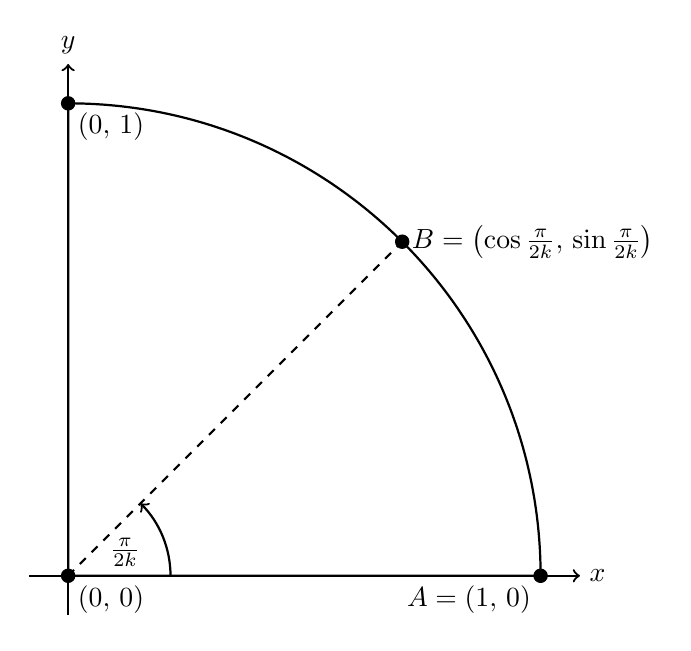
\begin{tikzpicture}[%%
  axisStyle/.style={->,thick},%%
  dashStyle/.style={-,dashed,thick},%%
  lineStyle/.style={-,thick},%%
  nodeStyle/.style={draw,inner sep=1.7pt,circle,fill=black,black}
]
%%
%%
%% The quadrant.
\pgfmathsetmacro{\angleEnd}{90}   %% angle in degrees
\pgfmathsetmacro{\angleStart}{0}  %% angle in degrees
\pgfmathsetmacro{\radius}{6}
%%
%% The axes.
\pgfmathsetmacro{\dx}{0.5}
\pgfmathsetmacro{\xhigh}{\radius+\dx}
\pgfmathsetmacro{\xlow}{-\dx}
\pgfmathsetmacro{\dy}{\dx}
\pgfmathsetmacro{\yhigh}{\radius+\dy}
\pgfmathsetmacro{\ylow}{\xlow}
%%
%% Some special points.
\coordinate (A) at (\radius,0);
\coordinate (B) at (4.24264068711929,4.24264068711929);  %% at 45 degrees
\coordinate (C) at (0,\radius);
\coordinate (origin) at (0,0);
%%
%% Draw a circle with an inscribed polygon.
\cartesianAxes
\myQuadrant
\end{tikzpicture}

\end{document}
